\begin{figure}[htbp]
\centering
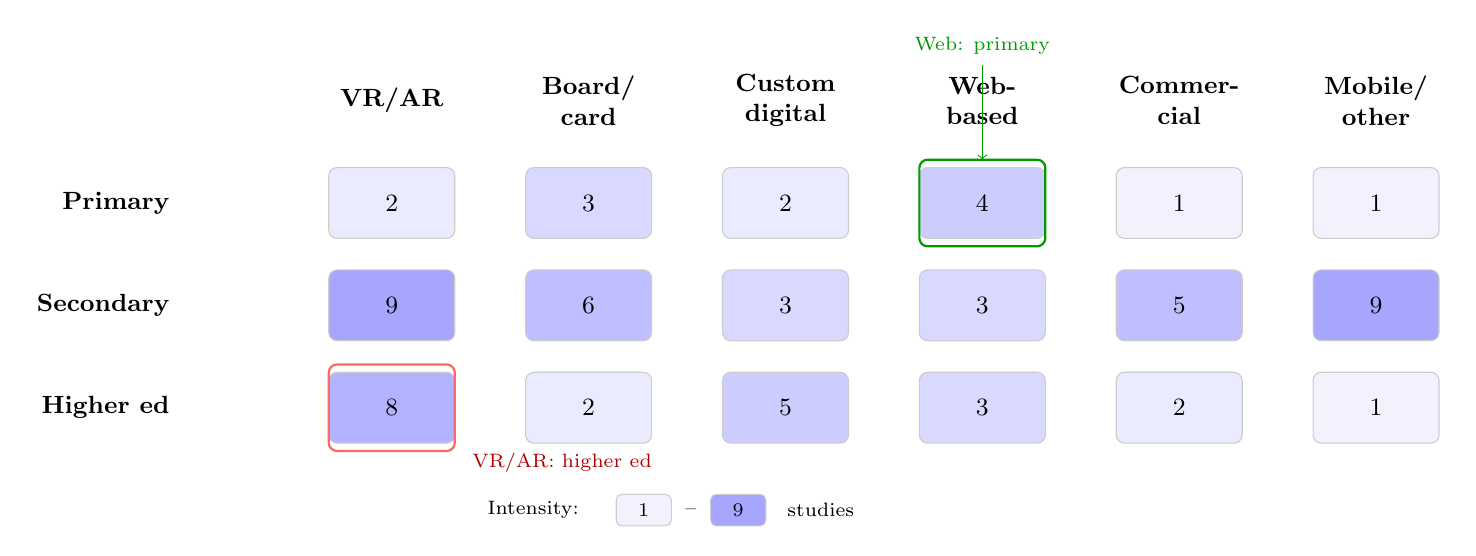
\begin{tikzpicture}[
    cell/.style={minimum width=1.6cm, minimum height=0.9cm, align=center, font=\small},
    hdr/.style={font=\small\bfseries, align=center, text width=1.6cm},
]

% Column spacing
\def\cs{2.5}  % column step

% Column headers
\node[hdr] at (0, 0) {};
\node[hdr] at (1*\cs, 0) {VR/AR};
\node[hdr] at (2*\cs, 0) {Board/\\card};
\node[hdr] at (3*\cs, 0) {Custom\\digital};
\node[hdr] at (4*\cs, 0) {Web-\\based};
\node[hdr] at (5*\cs, 0) {Commer-\\cial};
\node[hdr] at (6*\cs, 0) {Mobile/\\other};

% Row spacing
\def\rs{1.3}  % row step

% Row headers
\node[font=\small\bfseries, anchor=east] at (-0.2, -1*\rs) {Primary};
\node[font=\small\bfseries, anchor=east] at (-0.2, -2*\rs) {Secondary};
\node[font=\small\bfseries, anchor=east] at (-0.2, -3*\rs) {Higher ed};

% Primary row
\node[cell, fill=blue!8, draw=gray!40, rounded corners=3pt] at (1*\cs, -1*\rs) {2};
\node[cell, fill=blue!15, draw=gray!40, rounded corners=3pt] at (2*\cs, -1*\rs) {3};
\node[cell, fill=blue!8, draw=gray!40, rounded corners=3pt] at (3*\cs, -1*\rs) {2};
\node[cell, fill=blue!20, draw=gray!40, rounded corners=3pt] at (4*\cs, -1*\rs) {4};
\node[cell, fill=blue!5, draw=gray!40, rounded corners=3pt] at (5*\cs, -1*\rs) {1};
\node[cell, fill=blue!5, draw=gray!40, rounded corners=3pt] at (6*\cs, -1*\rs) {1};

% Secondary row
\node[cell, fill=blue!35, draw=gray!40, rounded corners=3pt] at (1*\cs, -2*\rs) {9};
\node[cell, fill=blue!25, draw=gray!40, rounded corners=3pt] at (2*\cs, -2*\rs) {6};
\node[cell, fill=blue!15, draw=gray!40, rounded corners=3pt] at (3*\cs, -2*\rs) {3};
\node[cell, fill=blue!15, draw=gray!40, rounded corners=3pt] at (4*\cs, -2*\rs) {3};
\node[cell, fill=blue!25, draw=gray!40, rounded corners=3pt] at (5*\cs, -2*\rs) {5};
\node[cell, fill=blue!35, draw=gray!40, rounded corners=3pt] at (6*\cs, -2*\rs) {9};

% Higher ed row
\node[cell, fill=blue!30, draw=gray!40, rounded corners=3pt] at (1*\cs, -3*\rs) {8};
\node[cell, fill=blue!8, draw=gray!40, rounded corners=3pt] at (2*\cs, -3*\rs) {2};
\node[cell, fill=blue!20, draw=gray!40, rounded corners=3pt] at (3*\cs, -3*\rs) {5};
\node[cell, fill=blue!15, draw=gray!40, rounded corners=3pt] at (4*\cs, -3*\rs) {3};
\node[cell, fill=blue!8, draw=gray!40, rounded corners=3pt] at (5*\cs, -3*\rs) {2};
\node[cell, fill=blue!5, draw=gray!40, rounded corners=3pt] at (6*\cs, -3*\rs) {1};

% Highlight annotations (outside the grid)
\draw[red!60, thick, rounded corners=3pt]
    (1*\cs-0.8, -3*\rs-0.55) rectangle (1*\cs+0.8, -3*\rs+0.55);
\node[font=\scriptsize, text=red!70!black, anchor=west] at (1*\cs+0.9, -3*\rs-0.7) {VR/AR: higher ed};

\draw[green!60!black, thick, rounded corners=3pt]
    (4*\cs-0.8, -1*\rs-0.55) rectangle (4*\cs+0.8, -1*\rs+0.55);
\node[font=\scriptsize, text=green!60!black] at (4*\cs, 0.7) {Web: primary};
\draw[green!60!black, thin, ->] (4*\cs, 0.45) -- (4*\cs, -1*\rs+0.55);

% Color scale legend (bottom, well separated)
\node[font=\scriptsize, anchor=east] at (2*\cs, -3*\rs - 1.3) {Intensity:};
\node[cell, fill=blue!5, draw=gray!40, rounded corners=2pt, minimum width=0.7cm, minimum height=0.4cm, font=\scriptsize] at (2*\cs+0.7, -3*\rs - 1.3) {1};
\node[font=\scriptsize] at (2*\cs+1.3, -3*\rs - 1.3) {--};
\node[cell, fill=blue!35, draw=gray!40, rounded corners=2pt, minimum width=0.7cm, minimum height=0.4cm, font=\scriptsize] at (2*\cs+1.9, -3*\rs - 1.3) {9};
\node[font=\scriptsize, anchor=west] at (2*\cs+2.4, -3*\rs - 1.3) {studies};

\end{tikzpicture}
\caption{Cross-tabulation of education level and game type across 74 studies: cell values indicate study counts, colour intensity reflects density (some studies span multiple categories)}
\label{fig:evidence-cross-dimensions}
\end{figure}
